\documentclass[10pt,a4paper]{article}

\usepackage[utf8]{inputenc}
\usepackage[T1]{fontenc}	
\usepackage[italian]{babel}
\usepackage{amsmath}
\usepackage{amsfonts}
\usepackage{amssymb}
\usepackage{graphicx}

\usepackage[left=2cm,right=2cm,top=2cm,bottom=2cm]{geometry}
\geometry{a4paper}

\usepackage{booktabs} % for much better looking tables
\usepackage{verbatim}
\usepackage{subfig} % make it possible to include more than one captioned figure/table in a single 

\usepackage{fancyhdr} % This should be set AFTER setting up the page geometry
\pagestyle{fancy} % options: empty , plain , fancy
\renewcommand{\headrulewidth}{0pt} % customise the layout...
\lhead{}\chead{}\rhead{}
\lfoot{}\cfoot{\thepage}\rfoot{}

%%% SECTION TITLE APPEARANCE
\usepackage{sectsty}
%\allsectionsfont{\sffamily\mdseries\upshape} % (See the fntguide.pdf for font help)
% (This matches ConTeXt defaults)
% pacchetti che mi fanno schifo ma uso lo stesso (Bob è scemo...)
\usepackage[cdot, thickqspace, squaren]{SIunits}
% macro che mi piacciono
\def\code#1{\texttt{#1}}


\title{Esercitazione 3: Misure DC su transistor e NOT TTL}

\author{Gruppo BE \\ Alessandro Candido, Roberto Ribatti}
\date{\today}
\begin{document}
\maketitle

\section{Scopo e strumentazione}
Lo scopo dell'esperienza era:
\begin{itemize}
\item familiarizzare con il funzionamento di un transistor BJT, le sue caratteristiche tensione-corrente e i vari regimi in cui può essere utilizzato (saturazione, attivo, interdizione);
\item costruire una porta NOT e  verificarne il funzionamento: studiare il circuito, l'effetto dei suoi componenti sul funzionamento e osservare i suoi limiti in frequenza.
\end{itemize}

Nella prima parte dell'esperienza si è inoltre osservata la dipendenza della corrente di collettore da $V_{CE}$, in regime attivo, cioè il cosiddetto Effetto Early.

La strumentazione usata è quella presente sul banco di lavoro, più:
\begin{itemize}
\item transistor \code{2N1711} - transistor NPN;
\item trimmer da $\unit{\sim 100}{\kilo\ohm}$;
\item stabilizzatore di tensione \code{LM7805}.
\end{itemize}

\section{Misure in DC sul transistor}
Si è proceduto alla realizzazione del circuito in figura \figurename{\ref{circuito}} con le componenti indicate.
\begin{figure}[h!]
\begin{minipage}[c]{0.25\textwidth}
\begin{align*}
R_L &= \unit{989 \pm 9}{\ohm}\\
R_B &= \unit{46.4 \pm 0.5}{\kilo\ohm}\\
R_{trim} &= \unit{101.5 \pm 0.9}{\kilo \ohm}\\
V_1 &= \unit{9.84 \pm 0.4}{\volt}\\
\end{align*}
	\end{minipage}
	\begin{minipage}[c]{0.3\textwidth}
	\centering
	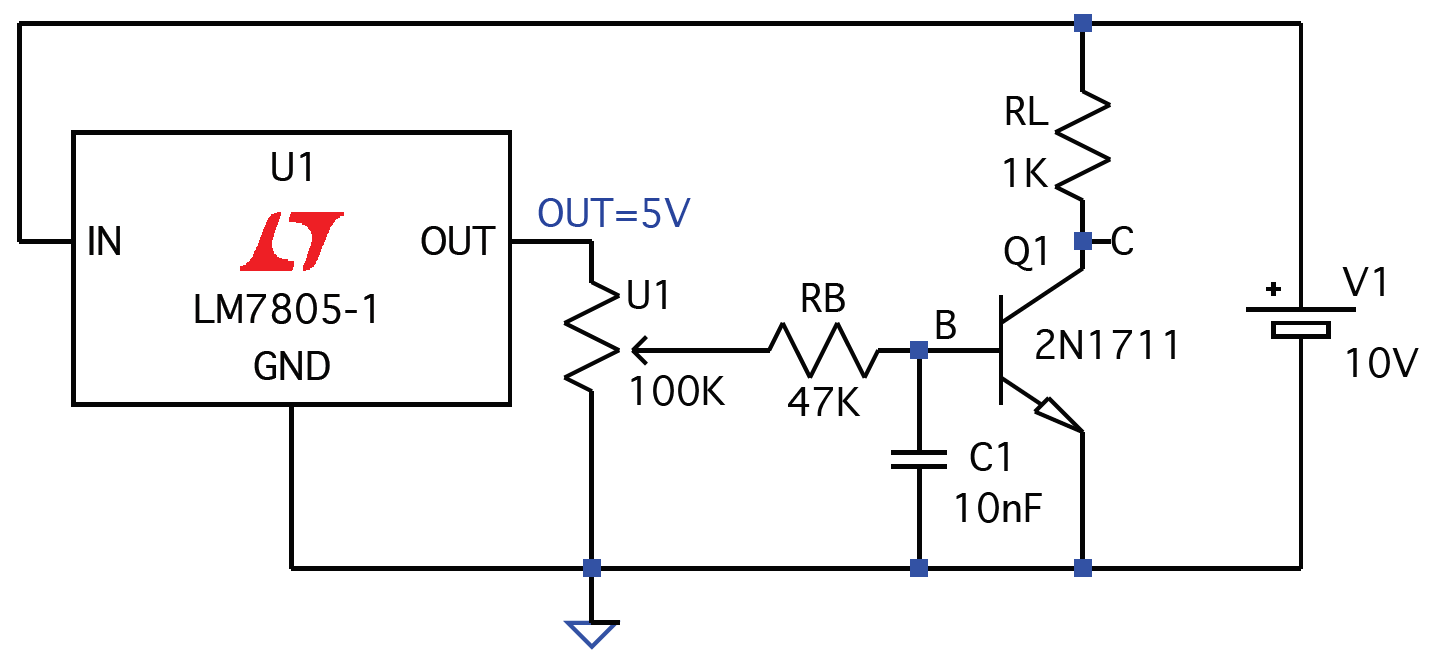
\includegraphics[width=1\textwidth]{../grafici/circuito.png}
	\caption{Circuito realizzato}
	\label{circuito}
	\end{minipage}
	\begin{minipage}[c]{0.45\textwidth}
		\centering
		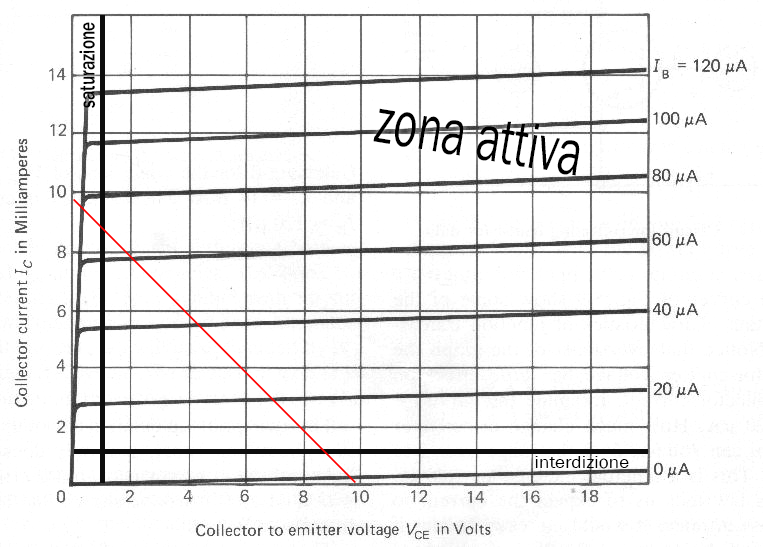
\includegraphics[width=1.1\textwidth]{../grafici/retta_carico.png}
		\caption{Retta di carico e zone di lavoro del transistor}
		\label{retta_carico}
	\end{minipage}
\end{figure}

Si è tracciata in \figurename{\ref{retta_carico}} la retta di carico sul grafico $I_c/V_{CE}$ fornito e si sono identificate le zone di interdizione (in basso), saturazione (a sinistra) e la zona attiva (il resto del grafico).
\\\\
\subsection{Misura di $I_C$ in funzione di $I_B$ e $V_{BE}$}
Si è proceduto alla misura di 3 tensioni al variare della posizione del potenziometro:
\begin{itemize}
	\item tensione base/emettitore $V_{BE}$ (misurata con l'oscilloscopio)
	\item tensione collettore/emettitore $V_{CE}$ (misurata con l'oscilloscopio), a partire dalla quale, nota la tensione di alimentazione $V_1$, si è calcolata la caduta di potenziale su $R_L$ e di conseguenza la corrente di collettore $I_C$;
	\item caduta di tensione su $R_B$ (misurata con il multimetro), con la quale si è calcolata la corrente di base $I_B$.
\end{itemize}
Si sono graficate la corrente di collettore $I_C$ in funzione della corrente di base $I_B$ e della tensione base/emettitore $V_{CE}$.
Di seguito riportiamo i dati raccolti e i grafici realizzati.

\begin{figure}[h!]
	\centering
	\begin{minipage}[h!]{0.40\textwidth}
		\centering
		\resizebox{1\textwidth}{!}{
			\input{../tabelle/tab_ib_var.txt}}
		\captionof{table}{Dati raccolti}
	\end{minipage}
	\begin{minipage}[d]{0.59\textwidth}
		\centering
		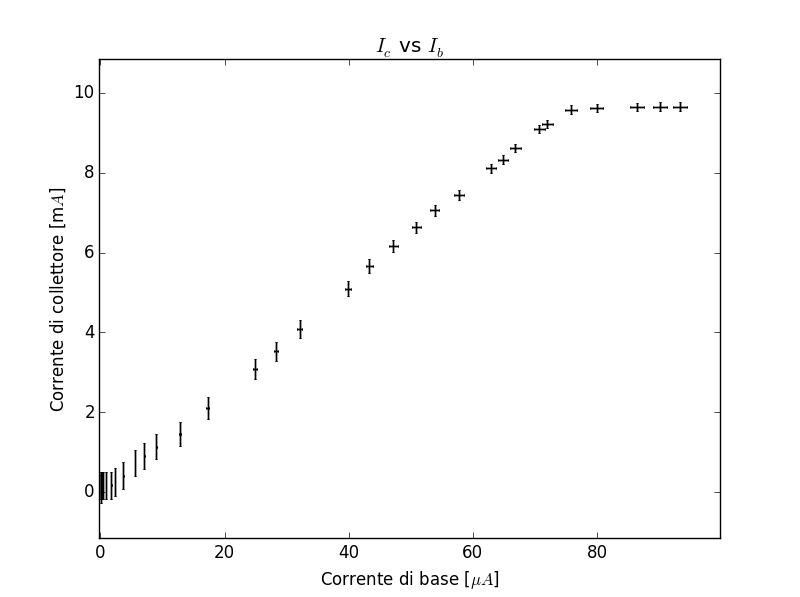
\includegraphics[width=1\textwidth]{../grafici/ic_ib.pdf}
		\caption{Grafico corrente collettore vs corrente di base}
		\label{ibic}
		\centering
		\includegraphics[width=1\textwidth]{../grafici/ic_vbe.pdf}
		\caption{Grafico tensione BE vs corrente collettore}
		\label{vbeic}
		\end{minipage}
\end{figure}

Variare la posizione del potenziometro non cambia la retta di carico ma modifica la corrente di base, quindi cambia la curva la cui intersezione con la retta di carico produce il punto di lavoro del transistor.
Il grafico in \figurename{\ref{ibic}} può essere suddiviso in tre parti:
\begin{itemize}
	\item i punti addensati vicino allo $0$ sono le intersezioni della retta di carico con le curve a corrente di base $\sim \unit{ 0}{\micro\ampere}$ (zona di interdizione);
	\item nella zona centrale è chiaro un andamento lineare, in questa zona la retta di carico interseca le curve in zona attiva ed è verificata l'ipotesi di linearità attesa: $I_C = h_{FE}*I_B$;
	\item per valori di corrente di base $\gtrsim \unit{80}{\micro\ampere}$, il grafico abbandona l'andamento lineare della zona centrale e si stabilizza sul valore di tensione $V_{CE}(sat)$: per grandi variazioni di corrente di base non corrispondo significative variazioni di corrente di collettore, in questa zona la retta di carico interseca le curve in zona di saturazione. Come è visibile in \figurename{\ref{retta_carico}} superati gli $\unit{80}{\micro\ampere}$ le curve intersecano la retta di carico circa nello stesso punto.
\end{itemize}
La massima corrente erogabile dal transistor è $I_{max}=V_1/R_L$\footnote{stiamo trascurando la resistenza del transistor poichè siamo in regime di saturazione}, con gli attuali parametri otteniamo $I_{max}=\unit{9.9 \pm 0.1}{\milli\ampere}$. In questo caso $I_{max}$ è determinata dalla caduta di potenziale sulla resistenza che precede il transistor, in generale (per resistenze piccole) dipenderà anche dalla massima potenza dissipabile dal transistor.
% che meccia con il risultato sperimentale
Per stimare la tensione di saturazione $V_{CE}(sat)$ si è fatta una media pesata dei punti presi in regime di saturazione e ottengo $V_{CE}(sat)$=\unit{298 \pm 5}{\milli\volt}.

Si è eseguito un fit lineare\footnote{che tenesse conto anche dell'errore sulle ascisse, che per certi dati è paragonabile a quello sulle ordinate} della zona centrale per il calcolo del parametro $h_{FE}$, il cui risultato è stato:
\begin{equation*}
h_{FE} = 130.1 \pm 2.2
\end{equation*}
\begin{figure}[h!]
	\centering
	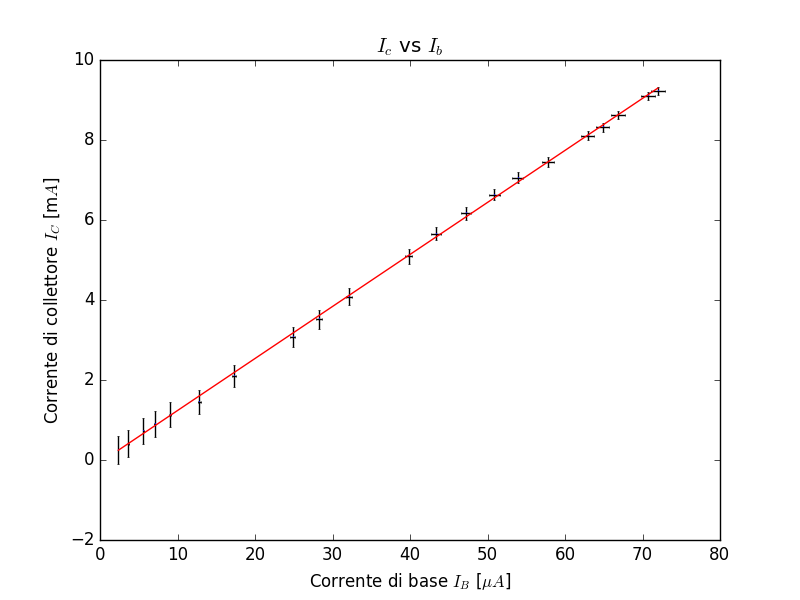
\includegraphics[width=0.6\textwidth]{../grafici/fit_h_fe.pdf}
	\caption{Grafico del fit di $h_{FE}$}
\end{figure}

Il grafico in \figurename{\ref{vbeic}} può essere diviso in due zone:
\begin{itemize}
	\item un plateau fino alla tensione di $\sim \unit{600}{\milli\volt}$, in questa zona troviamo i punti che nel grafico in \figurename{\ref{vbeic}} erano addensati vicino allo $0$, ovvero i punti di intersezione tra retta di carico e curve nella zona di interdizione.
	\item una retta molto pendente (o volendo un esponenziale in base al grado di approssimazione, come risulta dalle equazioni di Ebers-Moll) che parte come ci si aspetterebbe per $V_{BE} \sim \unit{0.7}{\volt}$, ovvero quando il transistor passa in zona attiva e la giunzione BE risulta polarizzata.
\end{itemize}

\subsection{Misura di $I_C$ in funzione di $V_{CE}$}
Si fissa adesso la posizione del potenziometro in modo da avere una corrente di base di $\sim \unit{40}{\micro\ampere}$. Si procede alla misura della tensione collettore/emettitore, $V_{CE}$, e della tensione di alimentazione, $V_1$, al variare di quest'ultima in un range tra $\unit{6}{\volt}$ e $\unit{15}{\volt}$.

Di seguito il grafico della corrente di collettore $I_C$\footnote{si è calcolata la caduta di tensione sulla resistenza $R_L$ per differenza delle due tensioni misurate} in funzione della tensione collettore/emettitore $V_{CE}$.

\begin{figure}[h!]
	\centering
	\begin{minipage}[h!]{0.3\textwidth}
		\centering
		\resizebox{\textwidth}{!}{
			\input{../tabelle/tab_Early.txt}}
		\captionof{table}{Dati raccolti}
	\end{minipage}
	\begin{minipage}[d]{0.69\textwidth}
		\centering
		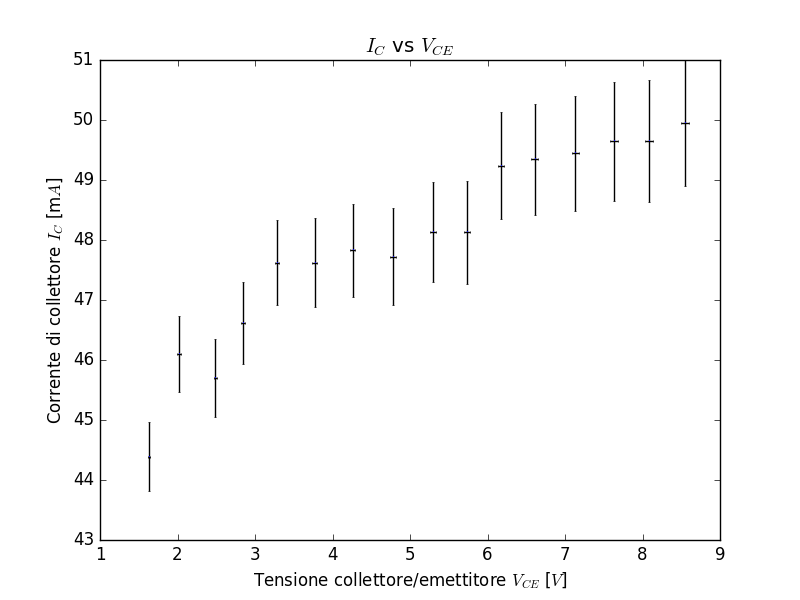
\includegraphics[width=\textwidth]{../grafici/fast_plot_Early.pdf}
		\caption{Grafico effetto Early}
		\label{early}
	\end{minipage}
\end{figure}

Al variare della tensione di alimentazione $V_1$ la retta di carico si muove parallelamente a se stessa sul grafico come in \figurename{\ref{retta_spostamento}}, quindi spostandosi la retta di carico interseca diversi punti della curva a  $\sim \unit{40}{\micro\ampere}$, il risultato e il caratteristico andamento lineare prodotto dall'effetto Early. Le misure effettuale sono rappresentate nel grafico in \figurename{\ref{early}} e sono affette da errori dovuti alla temperatura non costante del transistor che ne modificava il comportamento in maniera apprezzabile durante le misurazioni.

\begin{figure}[h!]
	\centering
	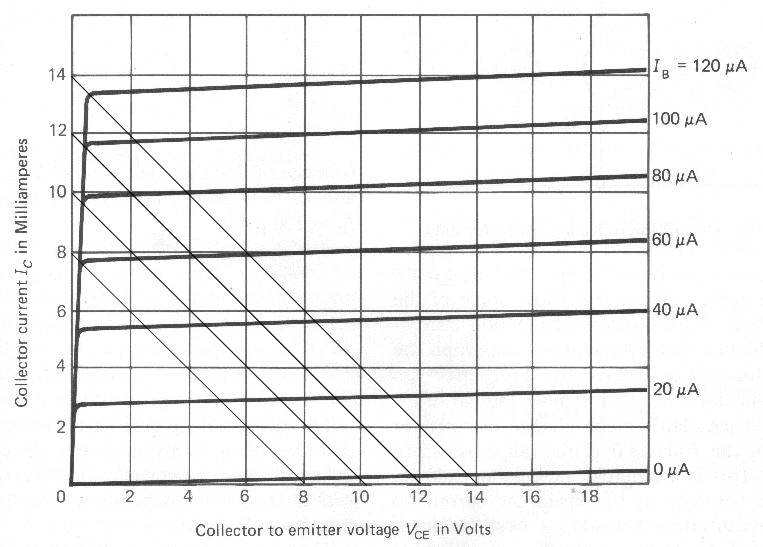
\includegraphics[width=0.54\textwidth]{../grafici/spostamento_retta.jpg}
	\caption{Variazione della retta di carico}
	\label{retta_spostamento}
\end{figure}
\section{Circuito NOT}

\subsection{Dimensionamento circuito e porta \code{NOT}}

% se torniamo in lab prendiamo una schermata del funzionamento come porta NOT dall'oscilloscopio
Si è costrituito il circuito riportato sulla scheda con i seguenti valori per le resistenze:
\begin{figure}[h!]
	\begin{minipage}[c]{0.5\textwidth}
		\begin{align*}
		R_1 &= \unit{15.20 \pm 0.13}{\kilo\ohm}\\
		R_2 &= \unit{99.4 \pm 0.9}{\kilo\ohm}\\
		R_L &= \unit{2.27 \pm 0.03}{\kilo\ohm}\\
		\end{align*}
	\end{minipage}
	\begin{minipage}[c]{0.5\textwidth}
		\centering
		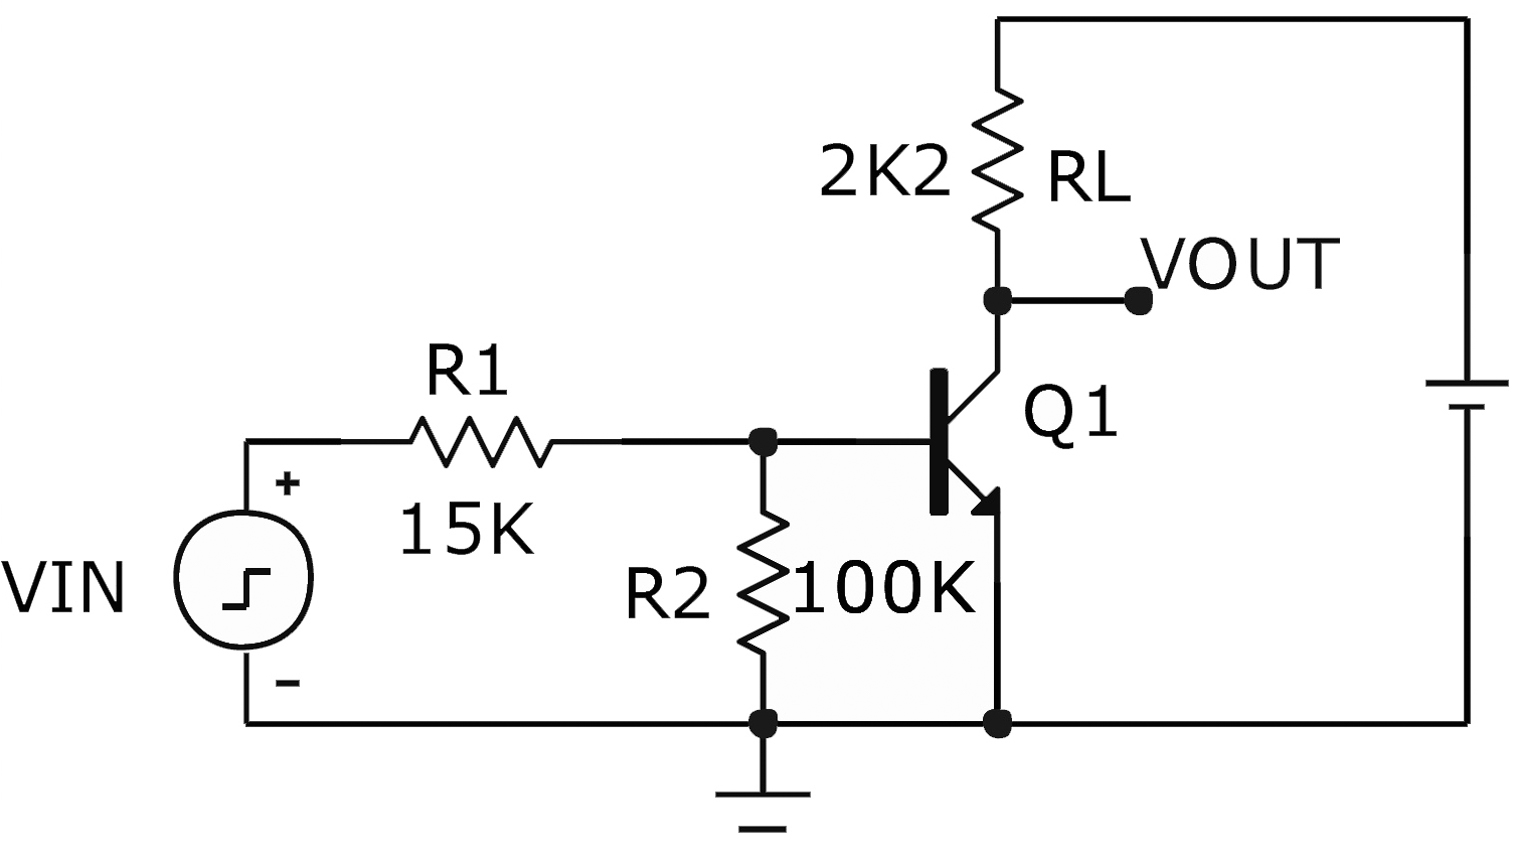
\includegraphics[width=0.8\textwidth]{../grafici/circuito_NOT.jpg}
		\caption{Circuito realizzato}
		\label{circuitoNOT}
	\end{minipage}
\end{figure}


L'alimentatore forniva una tensione pari a $\unit{5.07 \pm 0.04}{\volt}$.
Si sono quindi misurati i seguenti valori per gli stati \code{alto} e \code{basso} di $V_{out}$ e $V_{in}$:

\begin{table}[h!]
\centering
\begin{tabular}{c|c|c}
 & $V_{in}$ [mV]& $V_{out}$ [V]\\
\code{alto} & $668 \pm 20$ & $5.12 \pm 0.15$\\
\code{basso} & $0.24 \pm 0.10$ & $0.0576 \pm 0.0017$
\end{tabular}
\end{table}

Da cui si ottengono le correnti:
\begin{table}[h!]
\centering
\begin{tabular}{c|c|c}
 & $I_B$ [$\mu$A]& $I_C$ [mA]\\
\code{alto} & $278 \pm 18$ & $2.21 \pm 0.03$\\
\code{basso} & $0.329 \pm  0.013$ & $-0.022 \pm 0.025$
\end{tabular}
\end{table}
% ci riprovo, vediamo se funziona: (V_in - V_BE)/R1-V_BE/R2

Dal valore di $I_B$ è chiaro che il transistor lavora in regimedi saturazione/interdizione. Si è verificato che il circuito funzionasse come una porta \code{NOT}:

\begin{figure}[h!]
	\centering
	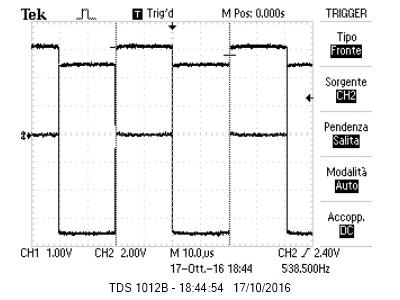
\includegraphics[width=0.45\textwidth]{../oscilloscopio/not_tarocco.jpg}
	\caption{Funzionamento porta NOT}
\end{figure}
\subsection{Ritardi}
Si è analizzato il comportamento del circuito su una scala temporale più piccola rispetto al periodo del segnale. Si nota che:
\begin{itemize}
\item il circuito produce un uscita non perfettamente in fase con l'ingresso;
\item l'onda quadra in uscita risulta non avere più un netto fronte di salita, ma impiega un tempo apprezzabile per cambiare stato.
\end{itemize}

Si sono misurati i tempi caratteristici, relativi ad una frequenza di input pari a $f = \unit{552 \pm 5}{\hertz}$, che vengono riportati di seguito. I nomi sono usati conformemente alla scheda relativa all'esercitazione. 

\begin{table}[h!]
\centering
\begin{tabular}{c|c|c|c}
$T_{rd} = \unit{264 \pm 5}{\nano\second}$ & $T_{d} = \unit{328 \pm 5}{\nano\second}$ & $T_{rs} = \unit{10.1 \pm 0.3}{\micro\second}$ & $T_{s} = \unit{1.98 \pm 0.03}{\micro\second}$
% ho inserito come errori solo gli 0.1DIV, non ricordo se vogliamo inserire anche una tacca/mezza-tacca addizionale del cursore in quadratura, oppure se in qualche misura c'era un po' di errore dovuto all'oscillazione della traccia
\end{tabular}
\end{table}
\paragraph{Discrepanza salita-discesa} Si nota che il tempo complessivo di discesa è 2 ordini di grandezza più grande di quello di salita. Si ricercano le cause di questa discrepanza nel funzionamento del transistor, e osservando il grafico $V_{CE} - I_C$ si nota che per compiere anche piccole variazioni di tensione lungo la retta di carico:
\begin{itemize}
\item per grandi tensioni $V_{CE}$, cioè in interdizione, il comportamento è quasi lineare, come in regime attivo;
\item per piccole tensioni $V_{CE}$, cioè in saturazione, per ottenere piccole variazioni sono necessarie grosse variazioni di $I_B$.
\end{itemize}
Si suppone che la variazione di $I_B$, che dovrebbe essere in fase con quella di $V_{in}$ (proveniente da \code{OUTPUT PULSE}), sia lineare,  ma anche tenendo conto di ciò si giustifica una differenza di tempi fra la parte vicina al basso sia della salita che della discesa, ma non la più evidente differenza tra i due.

% capacità per il fall time e densità di carica spaziale per storage time
% trovato qualcosa per spiegare lo storage time:
% https://en.wikipedia.org/wiki/Space_charge#Child.27s_Law
% https://www.researchgate.net/post/What_is_space_charge_limited_current

Considerando effetti di altro tipo si può però giustificare nei due casi il comportamento durante la variazione (cioè $T_{rs}$ e $T_{rd}$, non gli altri due). Quindi:
\begin{description}
\item[discesa] Il transistor deve transitare dallo stato alto allo stato basso, perciò deve passare da interdizione a saturazione. In interdizione si ha che la zona di svuotamento è piuttosto ampia e la carica che si accumula al suo interno lo rende una specie di condensatore. Perciò il tempo di discesa è dovuto a una configurazione molto simile alla scarica di un condensatore, per cui si deve considerare il tempo caratteristico in cui avviene tale scarica $\tau = R_L \cdot C_{ti}$ dove $C_{ti}$ è la capacità del transistor in interdizione. Essendo quest'ultima dell'ordine di $\sim \unit{100}{\pico\farad}$ \footnote{come riportato sul datasheet} si avrà una costante di tempo $\tau \sim \unit{100}{\nano\second}$.

\item[salita] Al contrario rispetto al caso precedente si deve passare da saturazione a interdizione. In questo caso si ha invece una regione di svuotamento molto ridotta (rispetto alle dimensioni "longitudinali"\footnote{Longitudinale nel modello a bacchetta, le equivalenti nel modello planare} della giunzione), perciò nel momento in cui si cerca di passare in interdizione si deve rimuovere tutti i portatori di carica che occupano la futura zona di svuotamento, e questo processo impiega un tempo non indifferente, denominato "storage time", che domina sul tempo di discesa dovuto a effetti capacitivi.
\end{description}

% manca ancora da giustificare T_rs

\subsection{Resistenza $R_2$}
Per osservare qualitativamente il comportamento del circuito al variare della resistenza $R_2$ si è sostituita quest'ultima con il trimmer, e si è variata la posizione del potenziometro visualizzando il comportamento nel dominio dei tempi sull'oscilloscopio.

Si è osservato che i tempi di salita e di discesa erano influenzati dall'entità della resistenza $R_2$, mentre i ritardi non subivano grosse variazioni in entrambi i casi.

Diminuendo la resistenza $R_2$ si ha che diminuisce anche la corrente $I_B$ che fluisce nella base del transistor, poiché una parte significativa della corrente proveniente da $V_{IN}$ finisce direttamente a terra tramite $R_2$. Infatti, schematizzando la giunzione BE come una resistenza costante $R_B$ (schematizzazione molto rozza, ma approssimativamente valida in regime attivo), si ha per la corrente $I_B$:
%è l'approsimazione di cavallo cilindrico, ma a meno che non la corregga Forti non la capiscono...
\begin{equation*}
I_B = \frac{V_{in} R_2}{(R_1 + R_2 // R_B)(R_2 + R_B)}
\end{equation*}
E quindi quando $R_1$ diventa dominante rispetto al parallelo e $R_B$ dominante rispetto a $R_2$ si ha che la corrente $I_B$ diminuisce.

Diminuendo $I_B$ l'oscillazione dello stato del transistor si avvicina sempre di meno alla zona di saturazione, con i seguenti effetti:
\begin{itemize}
\item Poiché la corrente di base è progressivamente limitata dall'alto, allora la tensione $V_{CE}$ non riesce a raggiungere valori troppo bassi, con un conseguente innalzamento del livello dello stato basso, cosa che si osserva.
\item Inoltre, diminuendo la massima corrente di base, diminuisce anche la massima corrente di collettore $I_C$ (la minima è già molto vicina a 0, si può considerare nulla) e questo cambia significativamente anche i tempi di salita e discesa, specie quello di salita che era dovuto all'accumulo di carica spaziale in saturazione.
\end{itemize}
% magari inserire i due numeri misurati

\subsection{Limiti del circuito in frequenza}
%inserire il numero trovato (5-10 kHz) e dare una spiegazione approssimativa di quanto accade
Si nota che il circuito funziona come porta \code{NOT} fino a una frequenza di circa $\unit{5-10}{\kilo\hertz}$. Oltre queste frequenze il segnale in uscita risulta molto deformato, al punto da non essere più identificabile con un'onda quadra.

Questo sembra essere dovuto al fatto che sebbene il segnale abbia un periodo minore, i tempi di latenza in salita risultano avere lo stesso ordine di grandezza di quanto misurato a frequenza più bassa, al punto che la transizione domina temporalmente sulla permanenza nello stato alto, che per frequenze troppo alte non si riesce neanche a raggiungere.

I limiti in frequenza del circuito in esame sono dunque dovuti ai tempi di latenza del transistor, nello specifico quelli in salita (da saturazione a interdizione).

\begin{figure}[t]
\centering
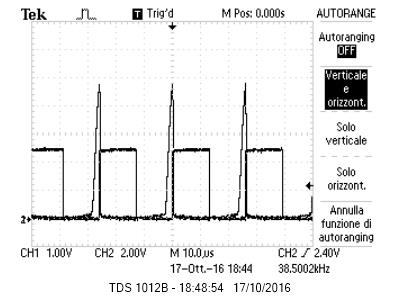
\includegraphics[width=0.5\textwidth]{../oscilloscopio/raise_problem.jpg}
\caption{Comportamento ad alte frequenze}
\end{figure}

\end{document}
